\documentclass[border=6pt]{standalone}
\usepackage[T1]{fontenc}
\usepackage{lmodern}
\usepackage{tikz}
\usetikzlibrary{arrows.meta,positioning,shapes.geometric,calc,fit}
\begin{document}
\hyphenpenalty=10000 \exhyphenpenalty=10000
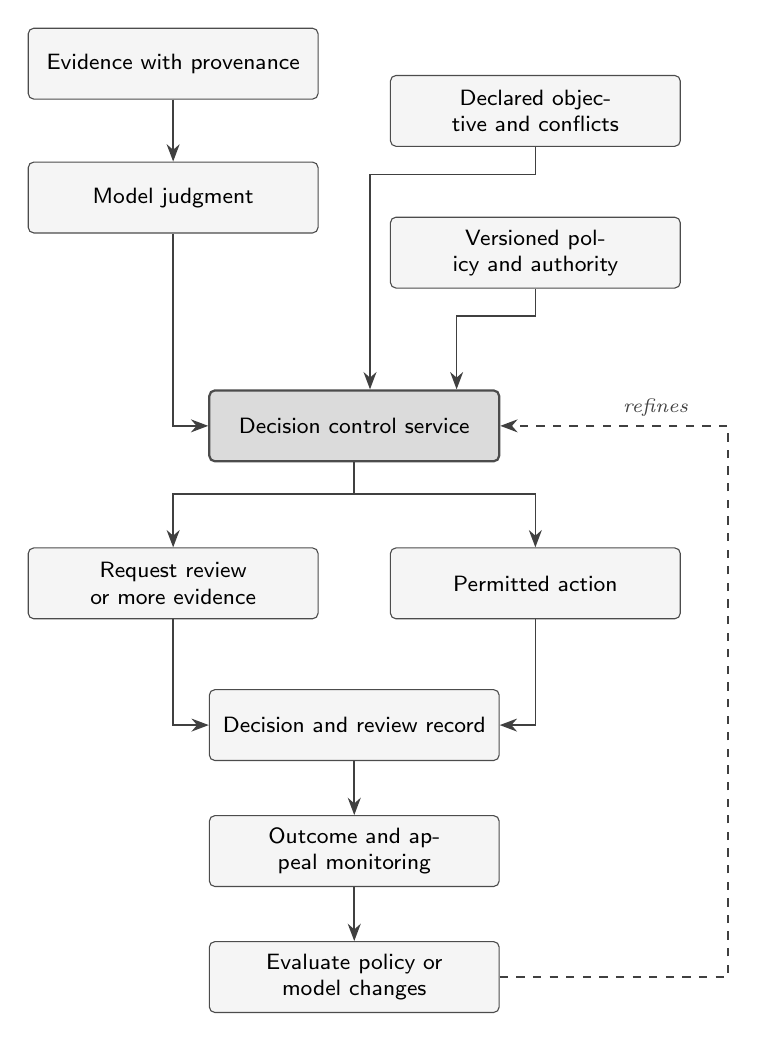
\begin{tikzpicture}[
  font=\footnotesize\sffamily,
  box/.style={draw=black!70, rounded corners=2pt, fill=black!4, align=center,
              text width=3.4cm, minimum height=0.9cm, inner sep=4pt},
  key/.style={box, fill=black!14, line width=0.8pt},
  arr/.style={-{Stealth[length=2.2mm]}, draw=black!75, line width=0.6pt},
  lab/.style={font=\scriptsize\itshape, text=black!75}
]
\node[box] (ev) at (-2.3,0) {Evidence with provenance};
\node[box] (mj) at (-2.3,-1.7) {Model judgment};
\node[box] (ob) at (2.3,-0.6) {Declared objective and conflicts};
\node[box] (po) at (2.3,-2.4) {Versioned policy and authority};
\node[key] (dcs) at (0,-4.6) {Decision control service};
\node[box] (rv) at (-2.3,-6.6) {Request review or more evidence};
\node[box] (ac) at (2.3,-6.6) {Permitted action};
\node[box] (rec) at (0,-8.4) {Decision and review record};
\node[box] (mon) at (0,-10.0) {Outcome and appeal monitoring};
\node[box] (evl) at (0,-11.6) {Evaluate policy or model changes};

\draw[arr] (ev) -- (mj);
\draw[arr] (mj.south) |- (dcs.west);
\draw[arr] (ob.south) -- ++(0,-0.35) -| ([xshift=0.2cm]dcs.north);
\draw[arr] (po.south) -- ++(0,-0.35) -| ([xshift=1.3cm]dcs.north);
\draw[arr] (dcs.south) -- ++(0,-0.4) -| (rv.north);
\draw[arr] (dcs.south) -- ++(0,-0.4) -| (ac.north);
\draw[arr] (rv.south) |- (rec.west);
\draw[arr] (ac.south) |- (rec.east);
\draw[arr] (rec) -- (mon);
\draw[arr] (mon) -- (evl);
\draw[arr, dashed] (evl.east) -- ++(2.9,0) |- (dcs.east) node[lab, above, pos=0.78, xshift=0.7cm] {refines};
\end{tikzpicture}
\end{document}
